\documentclass{revtex4-2}
\usepackage{physics,amsmath, amsfonts, siunitx, amssymb, graphicx, subcaption}
\usepackage[utf8]{inputenc}
\usepackage{hyperref}

% True/reconstructed parameters
\newcommand{\z}{\ensuremath{\cos{(\theta_z)}}}
\newcommand{\zreco}{\ensuremath{\cos{(\theta_z^{R})}}}
\newcommand{\ztrue}{\ensuremath{\cos{(\theta_z^{T})}}}
\newcommand{\treco}{\ensuremath{\theta_z^{R}}}
\newcommand{\ttrue}{\ensuremath{\theta_z^{T}}}
\newcommand{\xreco}{\ensuremath{x^R}}
\newcommand{\xtrue}{\ensuremath{x^T}}
\newcommand{\Ereco}{E^{R}}
\newcommand{\Etrue}{E^{T}}

% NSI parameters
\newcommand{\emm}{\ensuremath{\epsilon_{\mu\mu}}}
\newcommand{\emt}{\ensuremath{\epsilon_{\mu\tau}}}
\newcommand{\eet}{\epsilon_{e\tau}}
\newcommand{\eem}{\epsilon_{e\mu}}
\newcommand{\ett}{\ensuremath{\epsilon_{\tau\tau}}}
\newcommand{\ep}{\ensuremath{\epsilon^\prime}}

% Oscillation parameters
\newcommand{\dm}{\Delta m^2_{31}}
\newcommand{\sth}{\sin^2(2\theta_{23})}

% Neutrinos
\renewcommand{\ne}{\nu_e}
\newcommand{\nm}{\nu_\mu}
\newcommand{\ab}{\alpha\beta}
\newcommand{\nt}{\nu_\tau}
\newcommand{\ane}{\bar\nu_e}
\newcommand{\anm}{\bar\nu_\mu}               
\newcommand{\ant}{\bar\nu_\tau}

% Probabilities
\newcommand{\Pee}{P_{e  e}}
\newcommand{\Pem}{P_{e  \mu}}
\newcommand{\Pet}{P_{e  \tau}}

\newcommand{\Pme}{P_{\mu  e}}
\newcommand{\Pmm}{P_{\mu\mu}}
\newcommand{\Pmt}{P_{\mu  \tau}}

\newcommand{\Pte}{P_{P_{\tau e}}}
\newcommand{\Ptm}{P_{\tau  \mu}}
\newcommand{\Ptt}{P_{\tau  \tau}}

\newcommand{\Paeae}{P_{\bar{e}  \bar{e}}}
\newcommand{\Paeam}{P_{\bar{e}  \bar{\mu}}}
\newcommand{\Paeat}{P_{\bar{e}  \bar{\tau}}}

\newcommand{\Pamae}{P_{\bar{\mu}  \bar{e}}}
\newcommand{\Pamam}{P_{\bar{\mu}  \bar{\mu}}}
\newcommand{\Pamat}{P_{\bar{\mu}  \bar{\tau}}}

\newcommand{\Patae}{P_{\bar{\tau}  \bar{e}}}
\newcommand{\Patam}{P_{\bar{\tau}  \bar{\mu}}}
\newcommand{\Patat}{P_{\bar{\tau}  \bar{\tau}}}

\begin{document}
\section{Formalism of non-standard interactions}\label{sec:intro}
Non-standard interactions are sub-leading contributions to neutrino flavor transitions arising from neutrino interactions not considered in the Standard Model.
We consider matter NSIs arising from the neutral current NSIs, which exclude production 
and detection effects. An effective four-fermion Lagrangian for this type of interaction can be written as
\begin{align}
   \mathcal{L}_{\mathrm{NC}} &= -2 \sqrt{2} G_{F} \epsilon_{\alpha \beta}^{f X}\left(\bar{\nu}_{\alpha} \gamma^{\mu} P_{L} \nu_{\beta}\right)\left(\bar{f} \gamma_{\mu} P_{X} f\right)\,,
\end{align}
where NC denotes the neutral current interaction with 
$f \in \{e,u,d\}$, and $P_X$ is the chirality projection operators with $X \in \{L,R\}$.

For chirality $X$, the NSI Hamiltonian takes the form 
\begin{align}
   H &= \frac{1}{2E} UM^2U^\dagger + \sqrt{2}G_F n_e \text{diag}(1,0,0) + \sqrt{2}G_F \sum_f n_f \epsilon^{fX}\,,
\end{align}
where $U$ is the PMNS matrix, $M^2$ the matrix containing matter-squared differences, and $n_f$ the fermion number density
of fermion $f$.
We have no independent sensitivity for the chirality of $\epsilon^{fX}$, so we sum over these to obtain the vectorial parameter as $\epsilon^{fV}_{\alpha\beta} = \epsilon^{fL}_{\alpha\beta}+ \epsilon^{fR}_{\alpha\beta}$.
Moreover, we normalize $n_f$ by
the electron number density $n_e$. Our matter study will be wholly confined to the interior of the Earth, where we assume electrical neutrality and equal distribution of neutrons and protons, 
so we use the relations $n_u/n_e \simeq n_d/n_e \simeq 3$.
The effective NSI parameters in matter now take the form
\begin{align} \label{eq:epsilon}
    \epsilon_{\alpha\beta} &= \sum_{X \in \{L,R\}} \sum_{f \in \{e,u,d\}} \frac{N_f}{N_e} \epsilon^{fX}_{\alpha\beta} \nonumber \\
                           &= \sum_X \epsilon_{\ab}^{eX} + 3(\epsilon_{\ab}^{uX} + \epsilon_{\ab}^{dX})
\end{align}
We note that our definition of $\epsilon_{\alpha\beta}$ differs from e.g. \cite{deepcoreNSI}, where the quark number density is used to normalize
the parameters.

With the matter potential $V = \sqrt{2}G_F n_e$, we write
\begin{align} \label{eq:H_NSI}
   H &= \frac{1}{2E} UM^2U^\dagger + V\,
   \begin{bmatrix}      
      1 + \epsilon_{ee} & \epsilon_{e\mu} & \epsilon_{e\tau}  \\
      \epsilon_{e\mu} & \epsilon_{\mu\mu} & \epsilon_{\mu\tau}  \\
      \epsilon_{e \tau} & \epsilon_{\mu\tau} & \epsilon_{\tau\tau}
  \end{bmatrix}\,,
\end{align}
where we have assumed the components of the NSI matrix to be real. 

To propagate the neutrino states through the Earth, we solve the Schrödinger equation with the Hamiltonian from Eq.~\ref{eq:H_NSI}. 
The Earth density profile is taken from the PREM~\cite{PREM}, and we do not consider neutrino absorption.
The baseline for a given trajectory is determined using an average neutrino production height of 15 km and an Earth radius of 6371 km.
Thus, matter oscillations introduce a zenith angle dependence in two areas. Firstly, the matter potential depends on the matter density through the
neutrino propagates. A neutrino with indident zenith angle $\theta_z$ having $\z < -0.87$ will traverse through the dense Earth core, whereas a mantle-crossing neutrino 
with $\z > -0.87$ will not. Secondly, the zenith angle also alters the baseline through which a neutrino undergoes matter oscillations.
After this, we are ready to study the NSI effect on probability level.


\subsection{NSI phenomenology at probability level}\label{sec:nsiProbEffects}
% Since neutrinos and antineutrinos have different cross sections, they are treated separately in the detector simulations. 
% However, for the purpose of qualitatively elucidating the NSI effect in this subsection, we take the effective area of $\nm$ and $\anm$ to be equal. 
% Thus, we simply add the neutrino to the antineutrino contributions in both Fig.~\ref{fig:nsi_probs} and Fig.~\ref{fig:flux_ratio}.

% In the $\mu\tau$ sector, we have a resonance in the \SI{20}{\GeV} region. Any NSI parameter involving the $\mu$ or $\tau$ channel will dampen this resonance,
% with some also shifting the probability in the stationary region above \SI{100}{\GeV}.
% This `double effect' of both resonance dampening and shifting happens in two cases: either when the NSI parameter shares one channel with a survival probability
% (e.g. $\eem$ and $\Pmm$), or when the sectors align (e.g. $\emt$ and $P_{\mu\tau}$). The only exception to this is for $P_{\tau\tau}$, 
% which due to the near-maximal mixing in the $\mu\tau$ sector displays dampening for $\eem$ even though they share no channel directly. We illustrate
% the three different effects in Fig.~\ref{fig:nsi_probs}. 

% Due to the lightness of $\Delta m^2_{21}$, the $e$ channel has no resonance in the \si{\GeV} range. Thus, the only impact that 
% the NSI parameters considered here can have on any $\nu_e$ probability is shifting, and this only occurs when the requirements for the `double effect'
% are met. So except for the survival probability $P_{ee}$, any NSI parameter whose sector does not match the probability sector will not drastically affect it. 
% Thus, the only off-diagonal NSI parameters that strongly affect the transition probabilities $P_{\alpha\beta}$ are $\epsilon_{\gamma\beta}$,
% while the survival probabilities $P_{\alpha\alpha}$ are only strongly affected by $\epsilon_{\alpha\beta}$.

The atmospheric $\nm \to \nt$ transition is the most abundant, making $\emt$, $\emm$, $\ett$ the most suitable
NSI parameters to constrain from muon events. As we will see, $\eem$ is also a good candidate to constrain, albeit a weaker one. 

In Fig.~\ref{fig:emt_ett_probs}, we see how the introduction of $\emt = 0.02$ alters the $\nm$ and $\anm$ survival probabilities
for neutrinos that traverse the entire Earth diameter (i.e. $\z = -1$). $\emt$ does not dramatically change neither
amplitude nor frequency of the probabilities. Instead, it seems to stretch or compress the oscillations. Since the 
only difference between the way neutrinos and antineutrinos interact with matter is the sign of the potential, the probability for
$\nm$ with positive $\epsilon_{\alpha\beta}$ is identical to the probability for $\anm$ with negative $\epsilon_{\alpha\beta}$. Thus, the dashed line 
in the right panel not only shows the survival probability for $\anm$ with $\emt=0.02$, but also the survival probability for $\nm$ with $\emt=-0.02$.
Hence, we note that $\emt > 0$ stretches (compresses) $\Pmm$ for neutrinos (antineutrinos), while $\emt < 0$ compresses (stretches) $\Pmm$ for neutrinos (antineutrinos).

The value of $\ett$ affects neither $\Pmm$ nor $\Pamam$, in the IceCube region above \SI{500}{\GeV}. Hence, we will not be able
to say anything about $\ett$ in our IceCube study.  Comparing the probabilities in Fig.~\ref{fig:emt_ett_probs} with $\ett = 0.05$ with the ones for $\emt = 0.02$ in Fig.~\ref{fig:emt_ett_probs},
we see that even though we let $\ett$ take 2.5 times the value of $\emt$, its effect on $\Pmm$ is smaller. The weakening of the $\Pamam$ resonance will be visible in DeepCore, but we should expect a less stringent 
constraint due to the weakness of the effect compared to $\emt$. Thus, we will use IceCube to constrain $\emt$ only.

Moving on to $\eem$ and Fig.~\ref{fig:eem_eet_probs}, we see that both probabilities has shifted downwards for $\Etrue > \SI{500}{\GeV}$.
In Fig.~\ref{fig:eem_eet_probs}, we see that the muon channel remains largely unaffected of the value of $\eet$ as we expected. The exception of this lies 
in the DeepCore region of rapid oscillations, where mixing is more violent. 
\begin{figure} %TODO: maybe add shaded region > 500 GeV to signify IC limit
    \begin{center}
        \includegraphics[width=0.9\textwidth]{figures/Pmm_emt_probs.pdf}
        \includegraphics[width=0.9\textwidth]{figures/Pmm_ett_probs.pdf}
        \caption{\emph{Top panel:} Muon neutrino and antineutrino survival probabilities for
        $\z = -1$ when $\emt = 0.02$. All other NSI parameters are fixed to zero. In the \si{\GeV} range, $\emt$ shifts the oscillations to the right for $\nm$, and to the left for $\anm$. At \si{\TeV} energies, both probabilities simply get shifted down, resulting in a net reduction of track events.
        \emph{Bottom panel:} Muon neutrino and antineutrino survival probabilities for
        $\z = -1$ when $\ett = 0.05$. All other NSI parameters are fixed to zero. $\ett$ does not affect the probabilities above \SI{100}{\GeV} and this parameter is thus unable to be constrained by tracks in IceCube in our study. However, the dampening of the $\anm$ survival probability will be visible to DeepCore and PINGU, since it occurs within their energy ranges.}
        \label{fig:emt_ett_probs}
    \end{center}
\end{figure}

\begin{figure} %TODO: maybe add shaded region > 500 GeV to signify IC limit
    \begin{center}
        \includegraphics[width=0.9\textwidth]{figures/eem_probs.pdf}
        \includegraphics[width=0.9\textwidth]{figures/eet_probs.pdf}
        \caption{Muon neutrino and antineutrino survival probabilities for
        $\z = -1$. \emph{Top panel:} $\eem = 0.2$. All other NSI parameters are fixed to zero. Instead of the oscillations shifting to the left or right, $\eem$ dampens an oscillation peak for low \si{\GeV}. At \si{\TeV}, the probability is shifted down, just as with $\emt$.
        \emph{Bottom panel:} $\eet = 0.2$. All other NSI parameters are fixed to zero. Here, we see a very weak shifting and a $\nm$ weaker dip at low \si{\GeV}, and again, no visible effect at \si{TeV} energies. }
        \label{fig:eem_eet_probs}
    \end{center}
\end{figure}


%\begin{figure} %This one might be redundant with Fig 1 and 2
%   \includegraphics[width=0.85\textwidth]{figures/probabilities.pdf}
%   \caption{}\label{fig:nsi_probs}
%\end{figure}

The effect of NSI on the DeepCore event count has been previously discussed in~\cite{smirnovNSI}, while the NSI effect 
in PINGU has been studied in~\cite{choubey2014, ohlsson2013}.
Now we repeat our probability analysis but for the DeepCore/PINGU region of \SIrange{5.6}{56}{\GeV}. As we previously saw,
we have rapid oscillations, which means that `indirect' modifications (i.e. $\eet$ will affect the $\Pmm$ channel)
will be more apparent since all flavors are involved to a greater degree compared with the more stable region above \SI{500}{\GeV}, where 
many oscillations have averaged out.

Another feature of our DeepCore study includes the fact that we now have access to cascade events, in which $\ne$ and $\nt$ are more abundant.
Thus, we are no longer constrained to the $\mu$ channel alone, but we can now find interesting features in the other channels too. However, we 
remember that the $\nm$ flux is still the most abundant.

Fig.~\ref{fig:Pee_eet_probs} shows the electron neutrino and antineutrino survival probabilities, and here we see
a clear signal when turning on $\eet$. 

\begin{figure}
    \begin{center}
        \includegraphics[width=0.8\textwidth]{figures/Pee_eet_probs.pdf}
        \caption{Electron neutrino and antineutrino survival probabilities for
        $\ztrue = -1$ when $\eet = 0.2$. All other NSI parameters are fixed to zero. 
        Here we see a strong difference across the whole energy range, in contrast to the $\nm$ and $\anm$ plots in Fig~\ref{fig:eem_eet_probs}.}
        \label{fig:Pee_eet_probs}
    \end{center}
\end{figure}

Fig.~\ref{fig:emt_ett_probs} shows that $\emt$ affects both $\Pmm$ and $\Pamam$ over the whole energy range. Since 
IceCube also sees this, we hope to be able to boost the constraining of $\emt$ by combining the two experiments.

Regarding $\ett$ in Fig.~\ref{fig:eem_eet_probs}, the signal mainly shows in the $\Pamam$ channel as
a shallower dip in the \SI{20}{\GeV} region. Thus, DeepCore/PINGU alone will be used to constrain this parameter.

$\eem$ in Fig.~\ref{fig:eem_eet_probs} causes a weaker dip for both $\nm$ and $\anm$. 


For $\eet$, we see a similar effect on the dip in $\Pmm$ as we did with $\ett$ for $\Pamam$. Hence, we should be able to 
see the $\eet$ effect in DeepCore/PINGU. Remember that we now have the option to look at the other flavor channels than $\mu$ since we 
have cascade events for DeepCore and PINGU. If we simulate 
$\Pme^{NSI}$ at three different energies, and let both $\eem$ and $\eet$ vary together between the values $\{-0.3,0.3\}$, we produce a two-dimensional grid of probabilities.
Subtract the regular $\Pme^{SI}$ (i.e, $\Pme$ under standard interactions), and take the absolute value of the difference. We see the result in Fig.~\ref{fig:eem_eet_prob}. 
The middle and right panels, which show the absolute probability difference at \si{25} and $\SI{50}{\GeV}$, respectively, are very bleak,
indicating that the impact of the NSI parameters $\eem$ and $\eet$ is not as strong at these energy levels. Turning to the left-most panel,
we see a region in which the difference again is close to zero, but now surrounded by fringes of very large differences, up to $50\%$ difference 
in the $\Pme$ probability. This indicates that the NSI parameters are much more influential at these energies, and that we should be able to 
constrain both $\eem$ and $\eet$ from $\SI{5}{\GeV}$ cascade events.

\begin{figure}
    \centering
    \includegraphics[width=0.99\textwidth]{figures/eem_eet_prob.pdf}
    \caption{The quantity $\abs{P_{\mu e}^{NSI} - P_{\mu e}^{SI}}$ when we let $\eem$ and $\eet$ independently vary over
    the range \{$-0.3$, $0.3$\} at \si{5}, \si{25}, and $\SI{50}{\GeV}$. At $\SI{5}{\GeV}$, we see strong deviations in the probabilities, showing
    a promising indication that constriction of $\eem$ and $\eet$ is possible using cascade events at these energies.}\label{fig:eem_eet_prob}
\end{figure}

\subsection{NSI phenomenology at flux level}\label{sec:nsiFluxEffects}
To study the impact of NSI on the flux, we propagate the atmospheric neutrino flux from Honda et al~\cite{hondapaper} through the Earth.
The oscillation probability $P_{\alpha \beta}$ acts as a weight to the atmospheric flux, yielding the propagated flux for flavor $\beta$ at detector level as 
\begin{align}\label{eq:propFlux}
    \phi_\beta^\text{det} = \sum_\alpha P_{\alpha\beta} \phi_\alpha^\text{atm} \,,
\end{align}
where we sum over the initial lepton flavors $\alpha \in \{e,\mu, \bar{e}, \bar{\mu}\}$.
To illustrate the impact of $\emt$ at flux level, 
we plot in Fig.~\ref{fig:flux_ratio} the quantity $(\phi_{\nu_\mu}^{NSI} + \phi_{\bar\nu_\mu}^{NSI})/(\phi_{\nu_\mu}^{SI} + \phi_{\bar\nu_\mu}^{SI})$, 
where all fluxes are propagated to detector level by Eq.~\ref{eq:propFlux}.
In the left (right) panel, we plot the flux in region in which 99\% of the 
DeepCore (IceCube) track events originating from $\nm + \anm$ fluxes are contained. We see that the only clear signal discernible to the IceCube detector
is a energy-independent flux deficiency with a factor in the order of $\sim 10^{0.5}$ from core-crossing neutrinos within a zenith range of $\z < -0.87$. DeepCore on the other hand, 
is exposed to multiple fringes of flux surpluses with a factor in the order of $\sim 10$. The strongest surplus at \SI{20}{\GeV} is very weakly zenith dependent, a stark contrast to the
energy-independent but zenith-sensitive IceCube deficiency.
%TODO: check values above after final plot of flux ratios

The muonic flux not only carries the largest $\emt$ effect, but it is also more abundant than the $\ne$ flux. Thus, we expect to receive the highest statistics from $\mu$-related NSI parameters,
thus constraining them the strongest. $\epsilon_{\alpha\beta}$ which are only indirectly weakly dependent on the $\mu$ channel will have the weakest bounds. This could be improved
by considering cascade events in IceCube, thus opening up the $e$ and $\tau$ channels there.

\begin{figure}[!tb] %TODO: remove "true" in zenith x axis label?
   \begin{center}
      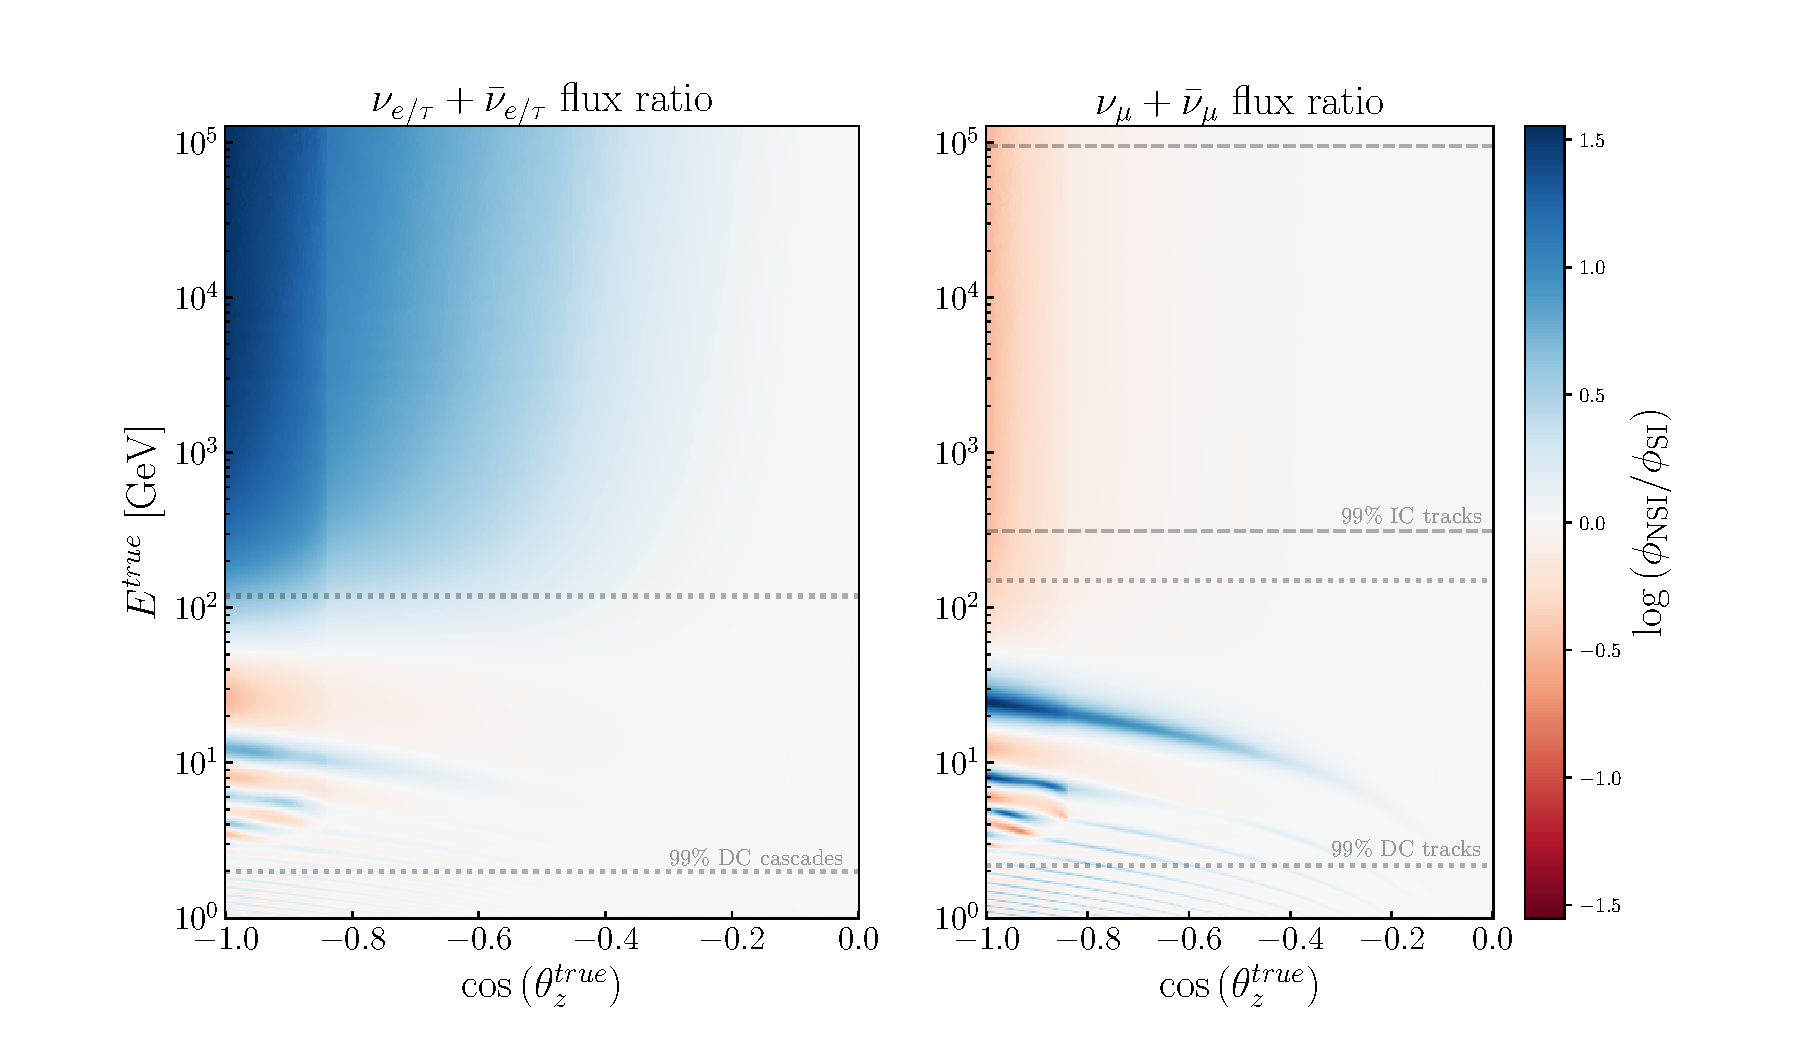
\includegraphics[width=0.99\linewidth]{figures/flux_ratio.pdf}
   \end{center}
   \caption{Ratio of atmospheric $\nu_\mu + \bar{\nu}_\mu$ fluxes at detector level, expressed as the logarithm of $(\phi_{\nu_\mu}^{NSI} + \phi_{\bar\nu_\mu}^{NSI})/(\phi_{\nu_\mu}^{SI} + \phi_{\bar\nu_\mu}^{SI})$.
   For the NSI fluxes $\phi^\text{NSI}$, we set $\emt = -0.05$, and all other $\epsilon_{\alpha\beta}=0$. For the SI fluxes $\phi^\text{SI}$, all $\epsilon_{\alpha\beta} = 0$.
   Left (right) panel shows the flux ratio in the energy range in which 99\% of the simulated DeepCore (IceCube) events are contained.
   }\label{fig:flux_ratio}
\end{figure}

\section{Detector formalism} %OK
The IceCube Neutrino Observatory is a gigaton Cherenkov detector located within Antarctic ice near the Geographic 
South Pole. It consists of 5160 individual digital optical modules situated on 86 strings, which detect Cherenkov light emitted by charged leptons
from neutrino events. We distinguish between two interaction topologies: track- and cascade-like events. Track-like events originate mainly
from muons originating from $\nm$ CC interactions, while cascades predominantly consist of electromagnetic and hadronic showers. 

DeepCore is a dense sub-array within the standard IceCube array, which allows us to observe neutrino interactions down to a few GeV~\cite{DC2021}.
Due to its lower energy threshold compared with IceCube, DeepCore has previously been used to study NSI effects in this more discernible range\cite{DC2021,deepcoreNSI}.

PINGU is a proposed 26 string in-fill array to IceCube, consisting of optical modules of similar nature~\cite{PINGUletter}. While proposed to mainly shed light on 
neutrino mass ordering, PINGU will be able to probe NSI parameters as well.  
\subsection{IceCube}\label{ch:ICmethod}

We obtain the data from the IC-86 sterile data release~\cite{IC2020}, which contains muon track events collected over 8 years. 
In the data, the reconstructed energy $\Ereco$ is logarithmically binned between \SI{500}{\GeV} to \SI{9976}{\GeV}, totalling 13 bins (index $i$).
The reconstructed cosine-zenith $\zreco$ is linearly binned between $-1$ and $0$ in 20 bins (index $j$). 

The event count for each bin reads
\begin{align}\label{eq:ICevents}
    N_{ij} = T \sum_\beta &\int_{(\zreco)_i}^{(\zreco)_{i+1}} \dd \zreco \int_{\Ereco_{j}}^{\Ereco_{j+1}} \dd \Ereco \times \nonumber \\
    \times &\int_0^\pi R(\treco,\ttrue) \dd \ztrue \int_0^\infty R(\Ereco,\Etrue) \phi_\beta^\text{det}  A^\text{eff}_\beta \dd \Etrue
    \,,
\end{align}
where $T$ is the live time of the detector, $\beta$ the final neutrino flavors, $\treco$ the reconstructed 
zenith angle, i.e.~the deduced direction of the incoming neutrino binned with index $i$. $\ttrue$ is the true zenith angle of the incoming neutrino. 
$\Ereco$ is the reconstructed energy, binned with index $j$. $R(\treco,\ttrue)$ is a zenith resolution function 
that describes the relationship with the reconstructed and true zenith angles, specific to the 86-string configuration of IceCube.
Similarily, $R(\Ereco,\Etrue)$ is the resolution function for the energy relationships. $\phi_\beta^\text{det}$ is the conventional atmospheric neutrino flux for flavor $\beta$, propagated to detector level
in accordance with Eq.~\ref{eq:propFlux}. The effective area $A^\text{eff}$ is binned and provided to us by the IceCube collaboration~\cite{ICaeff}.

For the energy and zenith resolution functions, we assume a log-normal distribution, giving it the form 
\begin{align}
    R(\xreco, \xtrue) = \frac{1}{\sqrt{2\pi} \sigma_{\xreco}\xreco} \exp\left[-\frac{(\log \xreco-\mu(\xtrue))^2}{2\sigma_{\xreco}^2}\right]\,.
\end{align}
However, the energy reconstruction is biased, meaning that the most probable reconstructed energy for a given true energy is not the same due to 
systematic differences~\cite{weaverThesis}. Thus, we don't assume that $\mu(\Etrue) =\Ereco$. 
To model this relationship between $\Etrue$ and $\Ereco$, we fit a Gaussian process regressor on the IC-86 Monte Carlo dataset from~\cite{IC2016}, from which
we can extract a predicted mean and standard deviation for a given $\Ereco$. We then take the $\Etrue$ points of the 99th percentile of each reconstructed
distribution to obtain the $\Etrue$ limits over which to integrate. We take the angular resolution function to be identically unity since the angle resolution in IceCube for track-like 
events is less than $\SI{2}{\degree}$, making $\ztrue$ practically coincide with $\zreco$ for our study~\cite{IC2020}. 

\subsection{DeepCore}\label{ch:DCmethod} % OK
We use the publically available DeepCore data sample~\cite{DC2019data} which is an updated version of what was used by the 
IceCube collaboration in a $\nu_\mu$ disapprearance analysis~\cite{DC2018mudisappearance}.

The detector systematics include ice absorption and scattering, as well as overall, lateral, and head-on optical efficiencies of the DOMs. 
They are applied as correction factors using the best-fit points from the DeepCore 2019 $\nu_\tau$ appearance 
analysis~\cite{DC2019tauappearance}.

The data include 14901 track-like events and 26001 cascade-like events, both divided into eight 
$ \log_{10}\Ereco \in [0.75,1.75]$ bins (index $i$), eight $\zreco \in [-1,1]$ bins (index $j$), and two bins for the event classification (index $k$). 
Each event has a Monte Carlo weight $w_{ijk,\beta}$ from which we can construct the event count as
\begin{align}\label{eq:MCevents}
    N_{ijk} &= C_{ijk}\sum_{\beta}w_{ijk,\beta}\, \phi_\beta^\text{det}\,,
\end{align}
where $C_{ijk}$ is the correction factor from the detector systematic uncertainty and $\phi_\beta^\text{det}$ is defined as Eq.~\ref{eq:propFlux}. 
We have now substituted the effect of the Gaussian smearing by treating the reconstructed and true quantities as a migration matrix. 

\subsection{PINGU}\label{ch:PINGUmethod} % OK
The methodology behind the PINGU simulations is the same as with our DeepCore study~\ref{ch:DCmethod}. We use the public Monte Carlo~\cite{PINGUdata}, 
which allows us to construct the event count as in Eq.~\ref{eq:MCevents}.
However, since no detector systematics is yet modeled for PINGU,the correction factors $C_{ijk}$ are all unity. We will remedy this by including an uncorrelated systematic error,
which we can scale at will.
As with the DeepCore Monte Carlo, the PINGU Monte Carlo is divided into eight 
$\log_{10}\Ereco \in [0.75,1.75]$ bins, and eight $\zreco \in [-1,1]$ bins for both track- and cascade-like events. 
We plot the normalized event differences $(N_{NSI} - N_{SI})/\sqrt{N_{SI}}$ for cascades and tracks in Fig.~\ref{fig:event_pulls}.
We generate `data' by predicting the event rates at PINGU with the following best-fit parameters from~\cite{nufit}, except for the CP-violating phase which is set to zero for simplicity.

\begin{align}\label{eq:PINGUparams}
    &\Delta m^2_{21} =  \SI{7.42e-5}{\electronvolt^2},\hspace{0.5em} \dm =  \SI{2.517e-3}{\electronvolt^2}, \nonumber \\
    &\theta_{12} = \SI{33.44}{\degree},\hspace{1em} \theta_{13} = \SI{8.57}{\degree},\hspace{1em} \theta_{23} = \SI{49.2}{\degree}, \hspace{1em} \delta_\text{CP} = 0\,.
\end{align}

\section{Results}
At the reconstructed event level, we note that the $\emt$ features discussed in Sec.~\ref{sec:nsiFluxEffects} display themselves differently in each detector.
%TODO: check that this is what is plotted.
$\epsilon^\pm_{\mu\tau} = \pm 0.01$.
Comparing the probability difference in Fig.~\ref{fig:Pmm_asymmetry} with the binned event count ratio in Fig.~\ref{fig:emt_events}, we see that the reconstruction of PINGU is
superior to DeepCore, since the event ratio $\log{(N^+_{NSI}/N^-_{NSI})} = \log{N^+_{NSI}} - \log{N^-_{NSI}}$ (in reconstructed quantities) 
more closely matches the probability difference $P^+-P^-$ (in true quantities).
This is most evident below \SI{20}{\GeV}, where the DeepCore reconstruction has washed out the fringes while PINGU preserves the $N^-_{NSI}$ surplus below \SI{10}{\GeV}.

Now we turn to the effect of $\emt$. %Muon events are the most abundant, and it suffices to study $\Pmm$ in this way to explain the $\emt$ features. 
As we see in Fig.~\ref{fig:emt_events}, the binned PINGU event counts display strong differences for many bins, which will give a high statistics on both sides of $\emt=0$, slightly favoring $\emt^-$. 
DeepCore on the other hand has fewer bins where the event count for $\emt^-$ surpasses the event count for $\emt^+$, 
giving weaker statistics for the negative side. Thus, we conclude that we will see a $\emt$ \si{GeV}-asymmetry stemming from the lower statistics 
for negative $\emt$ at probability level, which finally affects the reconstruction.

\begin{figure} % TODO: replace true -> T in labels
   \begin{subfigure}{1\textwidth}
      \begin{center}
      \includegraphics[width=0.5\linewidth]{figures/Pmm_asymmetry.pdf}
      \caption{$\Pmm(\emt^+) - \Pmm(\emt^-)$ using  $\emt^\pm = \pm 0.01$}\label{fig:Pmm_asymmetry}
      \end{center}
   \end{subfigure}
   \qquad
   \begin{subfigure}{0.99\textwidth}
      \includegraphics[width=1\linewidth]{figures/emt_events.pdf}
   \caption{The best-fit event count ratio from each detector for $\emt = \pm 0.01$. IceCube only observes a small surplus of events for $\emt=-0.01$ compared to 
   DeepCore and PINGU due to the weak NSI effect at high \si{\GeV} energies.}\label{fig:emt_events}
   \end{subfigure}
   \caption{Probability difference and best-fit event count. Negative $\emt$ has the strongest signal, as the thin blue 
   region stemming from $\emt = 0.01$ is less prominent than the red regions from $\emt=-0.01$.}
\end{figure}
 
\subsection{Constraining the NSI parameters}\label{sec:constraining} % Might need some shortening
In this section, we will constrain the four NSI parameters $\ett$, $\emt$, $\eem$, and $\eet$ by considering the detectors separately as well as jointly.
For our analyses, we define our $\chi^2$ as
\begin{align}\label{eq:chisq}
    \chi^{2}(\hat{\theta},\alpha,\beta, \kappa)=\sum_{ijk} \frac{\left(N^\text{th}-N^\text{data}\right)_{ijk}^{2}}
    {\left(\sigma^\text{data}_{ijk}\right)^{2} + \left(\sigma^\text{syst}_{ijk}\right)^{2}}+ 
    \frac{(1-\alpha)^2}{\sigma_\alpha^2} + \frac{\beta^2}{\sigma_\beta^2}\,
\end{align}
where we minimize over the model parameters $\hat{\theta} \in \{\dm, \theta_{23}, \epsilon\}$, the penalty terms $\alpha$ and $\beta$, and the free parameter $\kappa$.
$N_{ijk}^\text{th}$ is the expected number of events from theory in bin $\{i,j,k\}$, where $i$ denotes the $\Ereco$ bin, $j$ denotes the $\zreco$ bin,
and $k$ denotes the event-type bin, i.e. track or cascade. 
$N_{ijk}^\text{data}$ is the observed number of events in that bin. $\sigma^\text{data}_{ijk}$ is the experimental uncertainty, and $\sigma^\text{syst}_{ijk}$ the uncorrelated systematic
uncertainty.

In our simulations of $N_{ijk}^\text{th}$, we set all standard oscillation parameters to their current best-fit values of Eq.~\ref{eq:PINGUparams}, 
except for $\dm[31]$ and $\theta_{23}$
which we vary over their $3\sigma$ limits \SIrange{2.435e-3}{2.598e-3}{\eV\squared} and \SIrange{40.1}{51.7}{\degree}, respectively~\cite{nufit}.

We set $\sigma_\alpha = 0.25$ as the atmospheric flux normalization error, and $\sigma_\beta = 0.05$ as the zenith angle slope error~\cite{hondapaper}. 
The observed event number has an associated Poissonian uncertainty $\sigma_{ijk}^\text{data} = \sqrt{N_{ijk}^\text{data}}$.
For IceCube, the event count takes the form
\begin{align}
    N^\text{th}_{ij} = \alpha\left[1+\beta (0.5 + \zreco_i )\right] N_{ij}(\hat{\theta})\,,
\end{align}
with $N_{ij}(\hat{\theta})$ from Eq.~\ref{eq:ICevents}. Here, we allow the event distribution to rotate around the median cosine-zenith of $\zreco = -0.5$.

For DeepCore and PINGU, and the event count takes the form
\begin{align}
    N^\text{th}_{ijk} = \alpha\left[1+\beta \zreco_i \right] N_{ijk}(\hat{\theta}) + \kappa N_{ijk}^{\mu_{atm}}\,,
\end{align}
with $N_{ijk}(\hat{\theta})$ from Eq.~\ref{eq:MCevents}. $N_{ijk}^{\mu_{atm}}$ is the muon background, which is left to float freely in the DeepCore analysis.
The detectors experience an uncorrelated systematic error, which comes from the muon background, 
i.e. events misclassified as muons from 
$\nm$ interactions rather than from pion decay. For the DeepCore analysis, we will have to consider this background when calculating the events.
For IceCube events, we scan a higher energy range where the muon background can be neglected. For the PINGU events, the IceCube detector is 
expected to be able to act as a veto for this background. Thus, the error introduced from the muon background is expected by the collaboration 
to be negligible~\cite{PINGUletter}.
The background at PINGU can be considered negligible to first order~\cite{PINGUdata}, and we thus put $\kappa=0$ when calculating the PINGU $\chi^2$.
For DeepCore and PINGU, the median cosine-zenith is $\zreco = 0$, and we allow the event count to rotate around this point.

We treat the uncorrelated systematic uncertainties differently for each detector. For IceCube, we set $\sigma_{ij}^\text{syst} = f\sqrt{N_{ij}^\text{data}}$.
We consider best, normal, and worst-case scenarios in IceCube using
$f=5\%$, $10\%$, and $15\%$ respectively. For PINGU, we use the same form but instead use $f=0\%$, $3\%$, and $5\%$.
For DeepCore, we use the provided systematic error distribution which accounts for uncertainties in the finite MC statistics and the data-driven 
muon background estimate~\cite{DC2019data}. This is summarized in Table~\ref{table:syst_errors}.
{\renewcommand{\arraystretch}{1.2}
\begin{table}
   \centering
   \begin{tabular}{lccc}
      \hline \hline
      Experiment & Best case & Baseline & Worst case \\
      \hline
      IceCube & $5\%$ & $10\%$ & $15\%$ \\
      PINGU & $0\%$ & $3\%$ & $5\%$ \\
      \hline \hline
   \end{tabular}
   \caption{Our definition of the best, baseline, and worst case scenarios considered in each experiment, modelled by $\sigma_{ijk}^\text{syst} = f\sqrt{N_{ijk}^\text{data}}$ with $f$ from the table.
   We do not consider different DeepCore scenarios because her systematic error distribution is already provided in the data release~\cite{DC2019data}.}\label{table:syst_errors}
\end{table}

For the joint analysis, we follow the parameter goodness-of-fit prescription~\cite{maltoni2003} and construct the joint $\chi^2$ as 
\begin{align}\label{eq:joint_chisq}
    \chi^2_\text{joint} = \sum_\text{exp}\chi^2_\text{exp} - \chi^2_\text{exp,min}\,
\end{align}
with test statistic $\chi^2_\text{joint,min}$. The $\Delta \chi^2_\text{joint}$ is then $\Delta \chi^2_\text{joint} = \chi^2_\text{joint} - \chi^2_\text{joint,min}$.

We let each of the four NSI parameters considered assume a value, while keeping the other three fixed at zero. We consider the following ranges of values for each parameter:
\begin{align}
   -0.07 \le &\, \ett \le 0.07 \nonumber \\
   -0.03 \le &\, \emt \le 0.03 \nonumber \\
   -0.3 \le &\, \eem \le 0.3 \nonumber \\
   -0.3 \le &\, \eet \le 0.3 \nonumber \\
\end{align}

After the oscillation parameters $\dm[31]$ and $\theta_{23}$ have been marginalized out, we plot $\Delta \chi^2$ for each of the four NSI parameters in Fig.~\ref{fig:3D_NO}. 
The results are shown in Fig.~\ref{fig:IC_3D} and summarized in Tables~\ref{table:IC_DC_results} and~\ref{table:PINGU_joint_results}. Each region is bounded
by the best and worst-case scenario, as defined in Table~\ref{table:syst_errors}, while the middle line is the baseline scenario. We again emphasize that 
no uncertainty scenarios are considered for DeepCore, since they already provided in the data release~\cite{DC2019data}.

Comparing the PINGU and the DeepCore results in Fig.~\ref{fig:3D_NO}, we note that the best-fit for each NSI parameter for the PINGU experiment is expected to be zero. This is because the `data' we generated during 
the PINGU simulations assume no NSI since they have yet to be observed in nature. This introduces a non-NSI bias in all joint analyses, which include PINGU
since PINGU has stronger statistics than DeepCore and will thus pull the joint $\chi^2$ towards $\epsilon =0$.
Moreover, we see that we can expect PINGU to be sensitive to systematic uncertainty, especially when constraining $\eem$ and $\eet$ from the negative side.

\begin{figure}
    \begin{center}
       \includegraphics[width = 0.7\textwidth]{figures/joint_3D_NO.pdf}
       \caption{Confidence regions for PINGU and DeepCore scenarios listed in Table~\ref{table:syst_errors}, with their joint $\Delta \chi^2$ in maroon. $\dm[31]$ and $\theta_{23}$ and have been marginalized out, and all other NSI 
       parameters not shown in each panel are fixed to zero. 
       IceCube tracks only reveal $\emt$, and are displayed separately in Fig.~\ref{fig:IC_3D}. Dotted lines are the 90\% and $3\sigma$ CL levels.}\label{fig:3D_NO}
    \end{center}
 \end{figure} 
 \begin{figure}
    \begin{center} 
       \includegraphics[width=0.5\textwidth]{figures/PID_3D_emt.pdf}
       \caption{$\emt$ $\Delta \chi^2$ regions for scenarios as defined in Table~\ref{table:syst_errors}.
     $\dm[31]$ and $\theta_{23}$ and have been marginalized out, and all other NSI 
     parameters other than $\emt$ are fixed to zero. Dotted lines are the 90\% and $3\sigma$ CL levels.
     The zones contain the three uncertainty scenarios considered, and we see that the inclusion of PINGU is expected 
     to drastically make the bound on $\emt$ more stringent.
     }\label{fig:IC_3D}
    \end{center}
 \end{figure}
 
 {\renewcommand{\arraystretch}{1.0}
  \begin{table}
    \begin{center}
       \begin{tabular}{lcc}
          \hline
          Parameter & Best 90\% CL & Best $3\sigma$\\
          \hline & \multicolumn{2}{c}{IceCube}  \\
          $\emt$ &  [-0.012, 0.011] &  [-0.017, 0.016] \\\\
          & \multicolumn{2}{c}{DeepCore}\\ [0.3em]
          $\ett$ &  [-0.054, 0.067] &  [-0.089, 0.10] \\
          $\emt$ &  [-0.029, 0.0070] &  [-0.041, 0.026] \\
          $\eem$ &  [-0.12, 0.15] &  [-0.23, 0.24] \\
          $\eet$ &   [-0.084, 0.15] &  [-0.19, 0.21] \\\\
          &\multicolumn{2}{c}{IceCube + DeepCore} \\
          $\emt$ &  [-0.013, 0.0070] &  [-0.017, 0.013] \\
          \hline
          \vspace{2em}
       \end{tabular}
       \begin{tabular}{lcc}
          \hline
          Parameter & Baseline 90\% CL & Baseline $3\sigma$ \\
          \hline & \multicolumn{2}{c}{IceCube}  \\
          $\emt$ &  [-0.015, 0.014] &  [-0.022, 0.021] \\\\
          & \multicolumn{2}{c}{DeepCore}\\ [0.3em]
          $\ett$ &  [-0.054, 0.067] &  [-0.089, 0.10] \\
          $\emt$ &  [-0.029, 0.0070] &  [-0.041, 0.026] \\
          $\eem$ &  [-0.12, 0.15] &  [-0.23, 0.24] \\
          $\eet$ &   [-0.084, 0.15] &  [-0.19, 0.21] \\\\
          &\multicolumn{2}{c}{IceCube + DeepCore}\\
          $\emt$ &  [-0.016, 0.0070] &  [-0.022, 0.016] \\
          \hline
          \vspace{2em}
       \end{tabular}
       \begin{tabular}{lcc}
          \hline
          Parameter & Worst 90\% CL & Worst $3\sigma$\\
          \hline & \multicolumn{2}{c}{IceCube}  \\
          $\emt$ &  [-0.018, 0.017] &  [-0.025, 0.024] \\\\
          & \multicolumn{2}{c}{DeepCore}\\ [0.3em]
          $\ett$ &  [-0.054, 0.067] &  [-0.089, 0.10] \\
          $\emt$ &  [-0.029, 0.0070] &  [-0.041, 0.026] \\
          $\eem$ &  [-0.11, 0.15] &  [-0.23, 0.24] \\
          $\eet$ &   [-0.084, 0.15] &  [-0.188, 0.212] \\\\
          &\multicolumn{2}{c}{IceCube + DeepCore}\\
          $\emt$ &  [-0.018, 0.0070] &  [-0.024, 0.018] \\
          \hline
       \end{tabular}
       \caption{IceCube and DeepCore results from the $\Delta \chi^2$ in Fig.~\ref{fig:IC_3D}. $\dm[31]$ and $\theta_{23}$ have been marginalized out, and all other NSI parameters other than the one shown for each row are set to zero. Best, baseline, and worst refer to 
       the systematic uncertainty scenarios considered as in Table~\ref{table:syst_errors}.}\label{table:IC_DC_results}
    \end{center}
 \end{table}
 
 \begin{table}
    \centering
    \begin{tabular}{lcc}
       \hline
       Parameter & Best 90\% CL & Best $3\sigma$\\
       \hline & \multicolumn{2}{c}{PINGU} \\
       $\ett$ &  [-0.044, 0.051] &  [-0.062, 0.069] \\
       $\emt$ &  [-0.008, 0.009] &  [-0.014, 0.017] \\
       $\eem$ &  [-0.079, 0.081] &   [-0.16, 0.138] \\
       $\eet$ &  [-0.079, 0.098] &  [-0.148, 0.161] \\\\
       & \multicolumn{2}{c}{DeepCore + PINGU} \\
       $\ett$ &  [-0.036, 0.046] &  [-0.056, 0.064] \\
       $\emt$ &  [-0.0090, 0.0060] &  [-0.015, 0.013] \\
       $\eem$ &   [-0.060, 0.077] &  [-0.13, 0.13] \\
       $\eet$ &  [-0.052, 0.095] &  [-0.11, 0.14] \\\\
       & \multicolumn{2}{c}{IceCube + DeepCore + PINGU}  \\
       $\emt$ &  [-0.0080, 0.0050] &  [-0.012, 0.011] \\
       \hline
       %\vspace{0.5em}
    \end{tabular}
    \vspace{1em}
    \begin{tabular}{lcc}
       \hline 
       Parameter & Baseline 90\% CL & Baseline $3\sigma$\\
       \hline & \multicolumn{2}{c}{PINGU} \\
       $\ett$ &  [-0.046, 0.054] &  [-0.065, 0.073] \\
       $\emt$ &   [-0.0090, 0.010] &  [-0.015, 0.018] \\
       $\eem$ &  [-0.11, 0.094] &  [-0.20, 0.16] \\
       $\eet$ &   [-0.10, 0.11] &  [-0.19, 0.18] \\\\
       & \multicolumn{2}{c}{DeepCore + PINGU} \\
       $\ett$ &    [-0.038, 0.048] &  [-0.058, 0.067] \\
       $\emt$ &    [-0.010, 0.0060] &  [-0.016, 0.014] \\
       $\eem$ &    [-0.071, 0.086] &  [-0.15, 0.14]  \\
       $\eet$ &   [-0.061, 0.10] &  [-0.13, 0.16] \\\\
       & \multicolumn{2}{c}{IceCube + DeepCore + PINGU}  \\
       $\emt$ &  [-0.009, 0.0060] &  [-0.014, 0.012] \\
       \hline
       %\vspace{0.5em}
    \end{tabular}
    \begin{tabular}{lcc}
       \hline 
       Parameter & Worst 90\% CL & Worst $3\sigma$\\
       \hline & \multicolumn{2}{c}{PINGU} \\
       $\ett$ &  [-0.049, 0.057] &   [-0.07, 0.078] \\
       $\emt$ &   [-0.01, 0.011] &   [-0.017, 0.02] \\
       $\eem$ &   [-0.137, 0.11] &   [-0.228, 0.18] \\
       $\eet$ &  [-0.132, 0.125] &  [-0.226, 0.196] \\\\
       & \multicolumn{2}{c}{DeepCore + PINGU} \\
       $\ett$ &   [-0.039, 0.050] &    [-0.060, 0.070] \\
       $\emt$ &  [-0.011, 0.0070] &  [-0.017, 0.015] \\
       $\eem$ &  [-0.082, 0.097] &  [-0.168, 0.16] \\
       $\eet$ &  [-0.067, 0.11] &  [-0.15, 0.17] \\\\
       & \multicolumn{2}{c}{IceCube + DeepCore + PINGU}  \\
       $\emt$ &   [-0.010, 0.0060] &  [-0.016, 0.013] \\
       \hline
    \end{tabular}
    \caption{PINGU and joint results from the $\Delta \chi^2$ in Fig.~\ref{fig:3D_NO}. $\dm[31]$ and $\theta[23]$ have been marginalized out, and all other NSI parameters other than the one shown for each row are set to zero.
    Best, baseline, and worst refer to 
    the systematic uncertainty scenarios considered as in Table~\ref{table:syst_errors}.}\label{table:PINGU_joint_results}
 \end{table}
 
 
 \begin{table}
    \begin{center}
    \begin{tabular}{lccc}
            \hline \hline & \multicolumn{3}{c} {\text {Best fit}} \\
            \cline { 2 - 4 } Parameter & $\dm[31]$ & $\theta_{23}$  & $\epsilon$  \\
            \hline \multicolumn{3}{c} {\hspace{2.5cm} DeepCore }  \\[0.1em]
            $\ett$ &  2.435 & 47.84 & 0.0125 \\
            $\emt$ &  2.435 & 43.97 & -0.005 \\
            $\eem$ &  2.435 & 43.97 & 0 \\
            $\eet$ &  2.435 & 43.97  & 0.05 \\\\
            \multicolumn{3}{c} {\hspace{2.5cm} IceCube } \\
            $\emt$ &  2.435 & 51.70 & 0 \\
            \multicolumn{3}{c} {\hspace{2.5cm} IceCube + DeepCore } \\
            $\emt$ &  2.517 & 43.97 & -0.01 \\
            \hline
            \hline
    \end{tabular}
    \end{center}
    \caption{Best fit points for $\dm[31]$ and $\theta_{23}$ are given in units of $\si{10^{-3}\eV\squared}$ and
    degrees, respectively.}\label{table:bestfit}
 \end{table}
 
 We compare our results to a similar analysis performed on the same DeepCore dataset in~\cite{demidov}. In that publication, 
 the constraints found at 90\% CL were 
 \begin{align}\label{eq:demidov}
    -0.055 <&\, \ett < 0.056 \nonumber \\
    -0.023 <&\, \emt < 0.016 \nonumber \\
    -0.21 <&\, \eem < 0.20 \nonumber \\
    -0.19 <&\, \eet < 0.20\,.
 \end{align}
 Comparing~\ref{eq:demidov} to our results from Table~\ref{table:IC_DC_results} at 90\% CL, namely
 \begin{align}\label{eq:DC_results}
    -0.054 <&\, \ett < 0.067 \nonumber \\
    -0.029 <&\, \emt < 0.0070 \nonumber \\
    -0.12 <&\, \eem < 0.15 \nonumber \\
    -0.084 <&\, \eet < 0.15\,,
 \end{align}
 we see that our results for $\eem$, $\eet$ are more stringent, while the results for $\emt$ and $\ett$ are similar but more lenient. It is worth noting that the 
 results from~\cite{demidov} are have been obtained by including more systematic uncertainties, such as the spectral index, hadron production, and baryon resonance. 
 However, the overall flux normalization in~\cite{demidov} is 20\%, while we opted for a slightly higher figure of 25\%, which could compensate for the exclusion of the 
 statistical uncertainties mentioned.
 
 Using the baseline case of 3\% systematic uncertainty at 90\% CL, we find from Table~\ref{table:PINGU_joint_results}, that our predictions for the proposed PINGU detector are
 \begin{align}\label{eq:P_results}
    -0.049 <&\, \ett < 0.057 \nonumber \\
    -0.010 <&\, \emt < 0.011 \nonumber \\
    -0.137 <&\, \eem < 0.11 \nonumber \\
    -0.132 <&\, \eet < 0.125\,,
 \end{align}
 which displays an improvement over the DeepCore results in Eq.~\ref{eq:DC_results}, except for $\eet$ which is worse.
 
 Finally, the joint results for $\emt$ using IceCube and DeepCore from~\ref{table:PINGU_joint_results} at 90\% CL are
 \begin{align}\label{eq:ID_result}
    -0.016 <&\, \emt < 0.0070\,,
 \end{align}
 and when combining IceCube, DeepCore, and PINGU, the 90\% CL constraint on $\emt$ in our baseline scenario is predicted to be
 \begin{align}\label{eq:PID_result}
    -0.010 <&\, \emt < 0.0060\,,
 \end{align}
 which is more stringent for $\emt>0$ than the result in~\cite{deepcoreNSI}.
 
  \begin{figure}[t]
    \begin{center}
       \begin{subfigure}{0.44\textwidth}
          \includegraphics[width=1\linewidth]{figures/PINGU_event_pulls.pdf}
          \caption{PINGU}\label{fig:PINGU_event_pulls}
       \end{subfigure}
       \begin{subfigure}{0.54\textwidth}
          \includegraphics[width=1\linewidth]{figures/DC_event_pulls.pdf}
          \caption{DeepCore}\label{fig:DC_event_pulls}
       \end{subfigure}
     \end{center}
    \caption{Expected pulls of the form $(N_{NSI} - N_{SI})/\sqrt{N_{SI}}$ for PINGU and DeepCore after 3 years of data. 
    Each row has only one NSI non-zero parameter, with the first row having $\ett= -0.07$, second $\emt = -0.03$, third $\eem = -0.3$, and fourth $\eet = -0.3$.
    We clearly see the increased statistics of the PINGU detector, especially in cascade events. The low values of $\ett$ and $\emt$ produce a weak pull in DeepCore,
    while PINGU can be expected to observe multiple regions of strong pulls for $\emt$, $\eem$, and $\eet$.}\label{fig:event_pulls}
 \end{figure}
 
 We plot the event pull $(N_{NSI} - N_{SI})/\sqrt{N_{SI}}$ where $N_{(N)SI}$ are the numbers of expected events
 assuming (non-)standard interactions in Fig.~\ref{fig:event_pulls}. This gives the normalized difference in the
 number of expected events at the detector and illustrates the expected sensitivity of DeepCore for the NSI parameters.
 
 Now we will compare the probability plots with the final event counts in DeepCore. It is not enough to only study the effect at probability level, since that is in true quantities. 
 Since the detector data comes in reconstructed quantities, it might be the case that a feature at probability level gets averaged out in the reconstruction, and not showing up at all in the data. 
 In general, features showing at probability level are can be 
 averaged out at reconstruction if they occur in the rapidly oscillating part of single-digit \si{\GeV} energies. 
 
 The top right panel shows a surplus of DeepCore track events at \SIrange{20}{30}{\GeV} for through-going neutrinos when we turn on $\ett$. This is what we expected from the bottom right panel in Fig.~\ref{fig:emt_ett_probs}, where we saw that we had an increase in $\anm$ survival probability at \SIrange{20}{40}{\GeV}. 
 
 The third right panel shows the expected event pull for $\eem$. Comparing with the probabilities in Fig.~\ref{fig:eem_eet_probs}, we see that the surplus of the $\anm$ survival in the \SIrange{20}{30}{\GeV} and the deficit above \SI{40}{\GeV} is intact, while the \SI{10}{\GeV} $\nm$ deficit is completely averaged out.
 
 There is no reason for us to assume that only one NSI parameter exists in Nature, unless we impose a symmetry on the gauge group which generates NSI. So ideally, we would simulate a grid where all NSI parameters are allowed to vary, 
 but this is not feasible. Thus, we take we set $\ett = 0$ and let $\emt,\eem,\eet$ vary, along with $\dm[31]$ and $\theta_{23}$. We let $\ett=0$ because we saw that it did not influence the other parameters. 
 We then marginalize out the standard oscillation parameters and one of the NSI parameters and plot the remaining two in Fig.~\ref{fig:PINGU_2D}. We see that the pairs $\eem - \emt$ and $\eet - \emt$ are symmetrical. 
 Hence, we can see that no relationship exists between them. With $\eet - \eem$, however, the contours are assuming a different shape. The contour allows positive values of $\eet$ and $\eem$ to a greater degree than mixed or negative values.
 Thus, we can draw the conclusion that, given $\ett = 0$, PINGU might expect to observe that $\eem$ and $\emt$ are anti-correlated while we expect no significant correlation
 to be be seen between the pairs $\emt - \eem$, and $\emt - \eet$. This is consistent with our observation of the effect of these parameters on $\Pme$ in  Fig.~\ref{fig:eem_eet_prob}, from which we 
 saw that $\eem$ and $\eet$ strongly affect $\Pme$ for single-digit \si{\GeV} energies.
 
 \begin{figure}
    \centering
    \includegraphics[width=\textwidth]{figures/PINGU_2D_all_f0.pdf}
    \caption{Allowed regions for some of the NSI parameters after three years of PINGU data, assuming no uncorrelated systematic error. All plots are made with $\ett = 0$. The two
    standard oscillation parameters $\dm[31]$ and $\theta_{23}$ along with the one NSI parameter not shown have been marginalized out. We observe an anti-correlation between $\eem$ and $\eet$,
    consistent with our observation of the effect of these parameters on $\Pme$ in Fig.~\ref{fig:eem_eet_prob}.
    The values of the standard oscillation parameters 
    are taken from NuFit~\cite{nufit}.}\label{fig:PINGU_2D}
 \end{figure}

\subsection{Conclusion}\label{sec:conclusion}
We introduced Non-Standard Interactions (NSI) in Sec.~\ref{sec:intro} as a possible example of new physics beyond the Standard Model.
We then studied the effects of NSI on the neutrino oscillation probabilities and saw that NSI effects other than those stemming from $\emt$ are not apparent in the \si{\TeV} region.
Moreover, we saw in $\Pme$ that we could expect a correlation between $\eem$ and $\eet$ in the single-digit \si{\GeV} range.
We also saw that $\emt$ effects were visible on probability level in both the \si{\GeV} and \si{\TeV} regions.

We simulated the 86 string IceCube detector with track events, explained in Sec.~\ref{ch:ICmethod}.
In Sec.~\ref{sec:constraining}, we studied the NSI parameter $\emt$ and its effect events captured by IceCube. 
Using a $\chi^2$ test, we found that the bound from IceCube on $\emt$ at 90 \% confidence level was 
\begin{align}
    -0.015 <\,& \emt < 0.014\ \quad (90\% \text{ CL})
\end{align}
for our `baseline' case of 15\% uncorrelated systematic uncertainty.

In Sec.~\ref{ch:DCmethod}, we moved on and explained our method of simulating a second detector, DeepCore. Armed with simulations possible for this detector, we then continued to explore the possibility of NSI, this time including both track and cascade events and a lower energy region.
Using the $\chi^2$ test defined in Eq.~\ref{eq:chisq} and after marginalizing $\dm[31]$ and $\theta_{23}$ out, we found the following constraints on the NSI parameters at 90\% confidence level:
\begin{align}
    -0.054 <&\, \ett < 0.067 \nonumber \\
    -0.029 <&\, \emt < 0.0070 \nonumber \\
    -0.12 <&\, \eem < 0.15 \nonumber \\
    -0.084 <&\, \eet < 0.15\ \quad (\text{all at }90\% \text{ CL})\,.
 \end{align}
We compared these constraints to literature and found that the bounds for $\eem$ and $\eet$ were more stringent than those obtained in~\cite{demidov}.
Then, we did a joint $\chi^2$ test using simulated events from both IceCube and DeepCore. At 90\% confidence level, the bound of $\emt$ improved to
\begin{align}
    -0.016 <&\, \emt < 0.0070\ \quad (90\% \text{ CL})\,.
 \end{align}

In Sec.~\ref{ch:PINGUmethod} we described our method of simulating a proposed upgrade to the IceCube array: PINGU.
Since PINGU is not yet live, we produced data for it assuming a standard $3$ neutrino hypothesis with parameters from~\cite{nufit}.
After a $\chi^2$ analysis, we obtained the following constrains on the NSI parameters at 90\% confidence level:
\begin{align}
    -0.049 <&\, \ett < 0.057 \nonumber \\
    -0.010 <&\, \emt < 0.011 \nonumber \\
    -0.137 <&\, \eem < 0.11 \nonumber \\
    -0.132 <&\, \eet < 0.125 \quad (\text{all at }90\% \text{ CL})\,.
 \end{align}
After that, we did a joint $\chi^2$ analysis combining IceCube, DeepCore and simulated PINGU events to further constrict $\emt$. The bound at 90\% confidence level obtained was
\begin{align}
    -0.010 <&\, \emt < 0.0060\,. \quad (90\% \text{ CL})
 \end{align}

We were then able to draw the conclusion that we expect PINGU to successfully be able to observe the impact of NSI. Moreover, a joint analysis between PINGU and at least one of the other detectors under the IceCube collaboration
will be able to constrain the parameters even further. We saw that can expect PINGU to be more sensitive to NSI effects than DeepCore. We were also able to see that when constraining $\eem$ and $\eet$ from the negative side, 
we can expect the result to be highly dependent on the systematic uncertainty of PINGU.

Finally, we simulated the event count in PINGU, allowing $\emt$, $\eem$, and $\eet$ to vary, but setting $\ett=0$.
After and marginalizing out $\dm[31]$, $\theta_{23}$, and $\emt$, we saw that the effect of $\eem$ and $\eet$ on $\Pme$ had indeed propagated through to the event count,
manifesting as an anti-correlation between the $\eem$ and $\eet$ at both 90\% and $3\sigma$ confidence levels. No other pair of NSI parameters were observed to have 
a significant correlation.
\bibliographystyle{elsarticle-num}
\bibliography{article}

%\newpage
%\begin{tabular}{p{55mm}p{55mm}p{55mm}}
%    DeepCore (2017)
%       \begin{itemize}
%          \item[$\checkmark$] Honda atmospheric fluxes
%          \item[$\times$] Only look at tracks and $\emt$
%          \vspace{1em}  
%          \item[$\times$] DC Monte Carlo from an older dataset 
%          \item[$\times$] 8 E bins from $\SI{6.3}{\electronvolt^2}$ to $\SI{56}{\electronvolt^2}$
%          \item[$\times$] 8 z bins from -1 to 0 
%          \item[$\times$] Use "Overall" and "relative $\ne$ to $\nm$" normalization
%          \item[$\times$] Prior on spectral index
%          \item[$\times$] No zenith angle normalization
%          \item[$\checkmark$] No priors on $\dm, \theta_{23},\theta_{13}$
%       \end{itemize} &
%     Demidov (2020) DC analysis
%       \begin{itemize}
%          \item[$\checkmark$] Honda atmospheric fluxes
%          \item[$\checkmark$] Looks at tracks + cascades for $\emt$ and $\ett$
%          \item[$\checkmark$] Data and Monte Carlo from DC 2018
%          \item[$\checkmark$] 8 E bins from $\SI{5.6}{\electronvolt^2}   $ to $\SI{56}{\electronvolt^2}$
%          \item[$\checkmark$] 8 z bins from -1 to 1
%          \item[$\times$] Use "Overall" and "relative $\ne$ to $\nm$" normalization
%          \item[$\times$] Prior on spectral index
%          \item[$\times$] No zenith angle normalization
%          \item[$\checkmark$] No priors on $\dm, \theta_{23}$
%          \item[$\checkmark$] Fixes $\Delta m^2_{21}, \theta_{12}, \theta_{13}$
%          \item[$\times$] Uncertainty on hadron production in atmosphere
%          \item[$\times$] Uncertainty on neutrino nucleon cross section 
%       \end{itemize} &
%     This DC+PINGU analysis
%       \begin{itemize}
%          \item[$\checkmark$] Honda atmospheric fluxes
%          \item[$\checkmark$] Tracks and cascades for all flavors
%          \vspace{1em} 
%          \item[$\checkmark$] Reco $\to$ true mapping from Monte Carlo migration matrix
%          \item[$\checkmark$] 8 E bins from $\SI{5.6}{\electronvolt^2}$ to $\SI{56}{\electronvolt^2}$
%          \item[$\checkmark$] 8 zenith angle bins from -1 to 1
%          \item[$\checkmark$] Flux normalization uncertainty of 25\%
%          \item[$\checkmark$] Zenith angle uncertainty of 4\% 
%          \item[$\checkmark$] No priors on oscillation parameters 
%          \item[$\checkmark$] Marginalize $\dm$ and $\theta_{23}$. All other oscillation parameters are fixed.
%       \end{itemize} 
% \end{tabular}
\end{document}
